\section{Desarrollo}

\subsection{Herramientas utilizadas}

Para desarrollo del sniffer se analizaron las siguientes tecnologías:

\begin{itemize}
	\item Lenguajes: Python, C/C++, Java, Perl.
	\item libpcap, pycap, scapy.
	\item libnids, pynids.
	\item http\_parser.
	\item MySql, SQLite, PostgreSql, Oracle, Sql Server, SQLAlchemy.
	\item Mojolicious, Djando, Bottle, Web2py.
	\item ncurses.
	\item tinyproxy.
\end{itemize}

De esas herramientas nos decidimos en lenguaje por uno de bajo nivel. Y nos inclinamos por Python debido a que gran parte del grupo quería aprender a programar en dicho lenguaje o mejorar su experiencia de programación en el mismo. Su sintaxis además es simple y clara; dispone de tipado dinámico, de gran cantidad de librerías disponibles y es un lenguaje potente. Finalmente también otra punto a su favor es que es un lenguaje bastante usado en el ámbito del desarrollo ligado a la seguridad, con lo cual disponemos de gran variedad de librerías para utilizar.
\\
\\\indent En cuanto a las librerías de python relacionadas a la captura de tráfico que consideramos para realizar la implementación:

\begin{itemize}
\item PYCAP: es un módulo de bajo nivel que permite capturar e inyectar paquetes en cualquier interfaz de red, esta basada en libpcap y libnet. El principal problema que presenta es que solamente implementa hasta la capa TCP y no permite rearmar el flujo de la conversación TCP entre los hosts.
\item SCAPY: basada en PYCAP, es una implementación más modular que la anterior que permite definir de forma muy fácil nuevas capas. Si bien pudimos definir una capa para el tráfico HTTP, al igual que PYCAP, no permite de forma nativa rearmar los streams TCP.
\item PYNIDS: es una librería en python basada en libnids. A diferencia de las anteriores, PYNIDS emula el stack IP del kernel de Linux, ofrece defragmentación IP, ensamblado del stream TCP y detección de scaneo de puertos. Todo esto nos llevo a seleccionar esta librería.
\end{itemize}

Las 3 herramientas poseen la posibilidad de sniffear múltiples interfaces utilizando diferentes filtros para el tráfico. 
\\Se implementó un pequeño sniffer http con las 3 herramientas mencionadas. Si bien con todas ellas es bastante simple capturar tráfico, la mayor dificultad la encontramos al intentar rearmar el stream TCP, la única que puede realizar esto de forma nativa es PYNIDS. Por lo tanto en caso de querer utilizar PYCAP o SCAPY para nuestra implementación, deberíamos desarrollar por nuestra cuenta todo el ensamble y las conversaciones TCP entre los hosts. Por este último motivo elegimos PYNIDS.
\\Para interpretar y parsear la conversación HTTP se utilizarla librería http-parser, la cual soporta de forma completa la especificación de dicho protocolo. La misma posee una implementación en C, la cual posee una excelente performance a la hora de realizar su tarea.
\\Para la implementación de los diferentes plugins se utilizaron las respectivas versiones de las librerías para python (Sqlite, syslog, MySQLdb, etc). Se programaron una gran variedad de plugins, desde almacenamiento en bases de datos hasta notificaciones mediante correos electrónicos.
\\Y, finalmente, para implementar la aplicación web, usada para consultar los datos capturados por el sniffer, nos decantamos por el framework web Mojolicious debido a la experiencia con dicha herramienta por parte de uno de los miembros del grupo. Dicha aplicación solo trabaja con los datos generados en la base de datos SQLite.
\\
\\\indent Finalmente, se aclara que todo el trabajo fue desarrollado sobre Debian Linux.

\subsection{Diseño de la Aplicación}

Buscando alcanzar las características deseadas mencionadas anteriormente, decidimos dividir el sistema en tres grandes partes como se puede ver en el siguiente esquema (Sniffer, PluginManager y los plugins en sí):

\begin{figure}[hbtp]
    \centering
	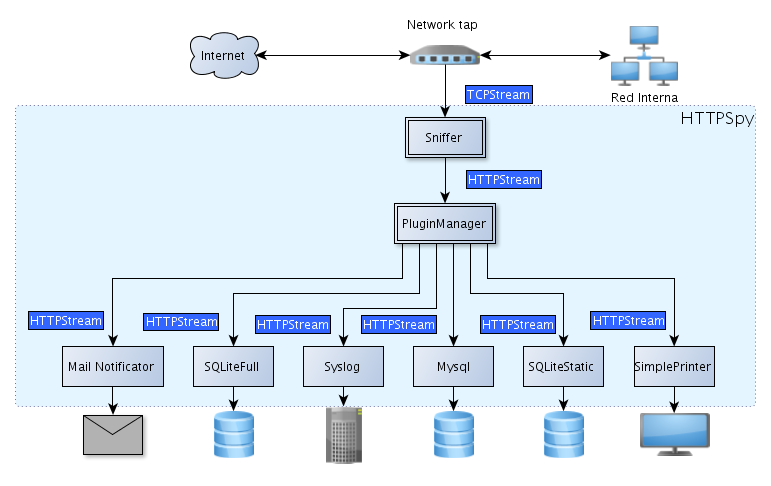
\includegraphics[width=\textwidth]{img/modelo.png}
\end{figure}

\subsubsection{HTTPSniffer}

Es el sistema de captura, es el encargado de capturar y extraer de las conversaciones HTTP/S la información relevante según las reglas de filtrado definidas. Por cada conversación HTTP genera una instacia de HTTPStream y ejecuta una función de callback definida pasándo dicho objeto como parámetro. Desde el punto de vista de diseño, simplemente es un singleton que wrapea la libreria pynids para facilitar levemente la interconexión entre las partes.

\begin{figure}[hbtp]
    \centering
	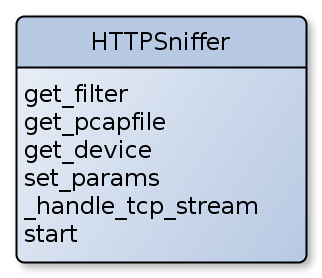
\includegraphics[scale=0.40]{img/HTTPSniffer.png} 
\end{figure}

\subsubsection{HTTPStream}

Representa una conversación HTTP, almacena toda la información interesante sobre la misma. No alacena el payload de la conversación. Para el parseo del flujo TCP se utiliza la librería http\_parser y luego se almacena la información relevante en colaboradores internos, los cuales pueden ser accedidos mediante una gran variedad de getters.

\begin{figure}[hbtp]
    \centering
	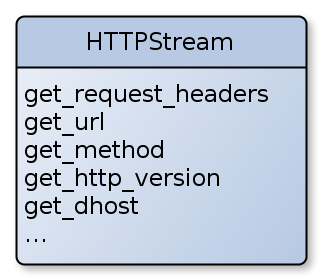
\includegraphics[scale=0.40]{img/HTTPStream.png} 
\end{figure}

\subsubsection{PluginsManager}

Administra los plugins instalados en la aplicación. Asocia el nombre del plugin con la clase correspondiente. Es responsabilidad de cada plugin de registrarse contra el PluginsManager para que forme parte del sistema y esta disponible para el usuario. Dicha registración se realiza por medio del método \textbf{register}.

\begin{figure}[hbtp]
    \centering
	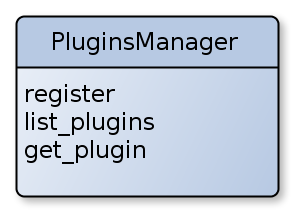
\includegraphics[scale=0.40]{img/PluginsManager.png} 
\end{figure}

\subsubsection{Plugins}

Son los encargados de procesar los requests capturados por el sniffer. Son objetos muy simples y el único requerimiento es que implementen los métodos \textbf{log\_stream} y \textbf{help}. 
\\\\
\newpage %se pasa a otra page porque quedaba solo el título al final de una página (si este hecho se modifica sacar toda esta línea)
\textbf{Plugins implementados:}
\begin{itemize}
	\item \textbf{SimplePrinter:} Este plugin imprime por stardard output, según un formato configurable, información sobre la conversacion HTTP.
	\item \textbf{SyslogPrinter: } Este plugin registra por Syslog, según un formato configurable, información sobre la conversacion HTTP.
	\item \textbf{SQLiteStatic:} Almacena en una unica tabla SQLite los siguientes campos: source host, destination host, request path, request method, status code, content length, content type.
	\item \textbf{SQLiteFull: } Almacena en tres tablas SQLite toda la información relacionada a la conversación, incluyendo todos los headers.
	\item \textbf{MySQLFull: } Almacena en tres tablas MySQL toda la información relacionada a la conversación, incluyendo todos los headers.
	\item \textbf{MailNotificator: } Envía por mail notificaciones de conexiones que cumplen ciertas condiciones críticas informadas. Envía datos tales como source host, destination host, source port, destination port, request url, request path, request method, status code, content type, content type, time of the request.
\end{itemize}

\begin{figure}[hbtp]
    \centering
	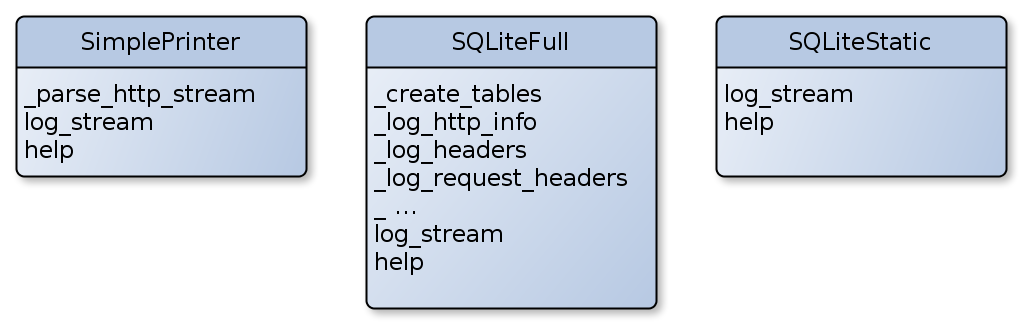
\includegraphics[scale=0.40]{img/Plugins1.png} 
\end{figure}

\begin{figure}[hbtp]
    \centering
	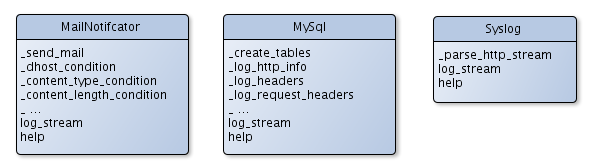
\includegraphics[width=\textwidth]{img/Plugins2.png} 
\end{figure}
